%------------------------------------------------------------------------
%Editar Diplomado
\hypertarget{cv:eliminarCU}{\section{Eliminar Caso de Uso}} \label{sec:eliminarCU}

	Esta funcionalidad le permitirá eliminar un caso de uso innecesario o incorrecto. Para eliminar una caso de uso es necesario que no se encuentre asociado a otros casos de uso, al igual que sus trayectorias y/o pasos.

		\subsection{Procedimiento}

			%Pasos de procedimiento
			\begin{enumerate}
	
			\item Oprima el botón \IUBotonEliminar{} de un registro existente de la pantalla \ref{fig:GestionarCU} ''Gestionar Casos de Uso''.
	
			\item Se mostrará el mensaje \ref{fig:confirmaEliminaCU} sobre la pantalla \ref{fig:GestionarCU} ''Gestionar Casos de Uso''.
			
			%Pantalla
			\begin{figure}[htbp!]
				\begin{center}
					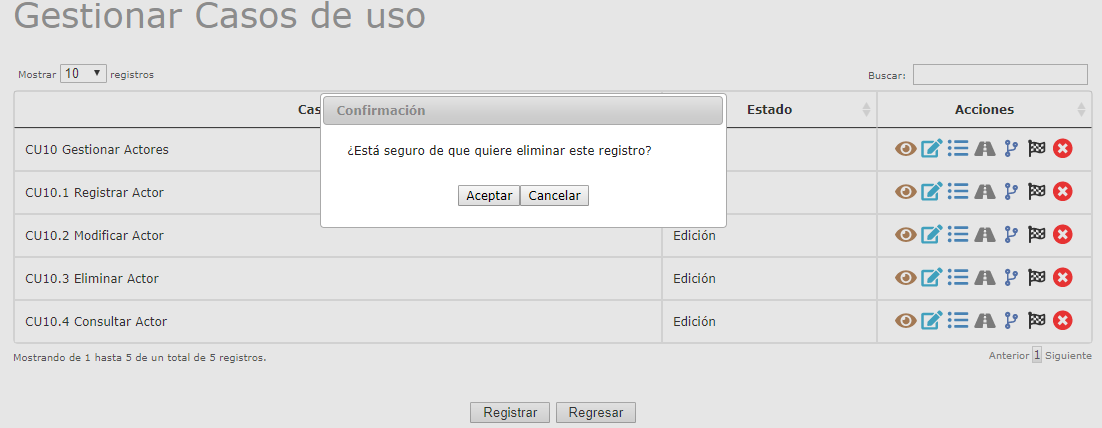
\includegraphics[scale=0.6]{roles/lider/casosUso/pantallas/IU12-3MSG10}
					\caption{MSG de Confirmación}
					\label{fig:confirmaEliminaCU}
				\end{center}
			\end{figure}
						
			\item Oprima el botón \IUAceptar.
			
			\item Se mostrará el mensaje \ref{fig:CUEliminado} en la pantalla \ref{fig:GestionarCU} ''Gestionar Casos de Uso''.
			
			\begin{figure}[htbp!]
				\begin{center}
					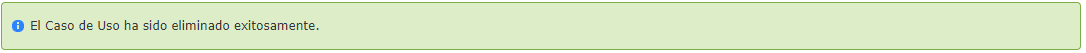
\includegraphics[scale=0.6]{roles/lider/casosUso/pantallas/IU12-3MSG1}
					\caption{MSG: Caso de Uso Eliminado}
					\label{fig:CUEliminado}
				\end{center}
			\end{figure}
			\end{enumerate}